Let's consider some observed posts.

Quoting \href{https://c.im/@nickheer/}{@nickheer@c.im}:
\url{https://c.im/@nickheer/111424148073619205} \#retoot

\begin{figure}
\centering
\pandocbounded{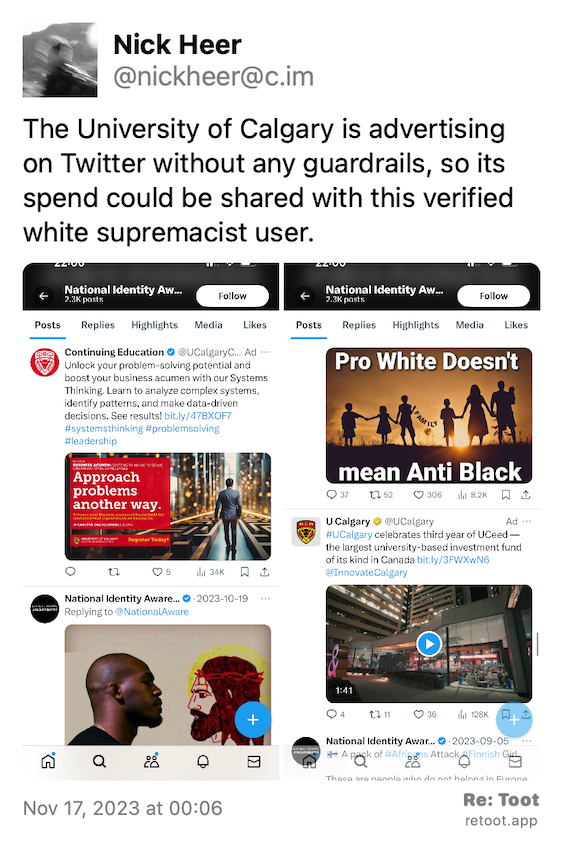
\includegraphics[keepaspectratio]{\%7B\%7Bsite.url\%7D\%7D/img/calgaryfail.jpg}}
\caption{Post by Nick Heer. ``The University of Calgary is advertising
on Twitter without any guardrails, so its spend could be shared with
this verified white supremacist user.'' The post contains media with the
following descriptions: An image described as: ``Screenshot of
University of Calgary ad appearing next to racist tweet from verified
account.'' An image described as: ``Screenshot of Twitter showing
University of Calgary ad in white supremacist feed.'' Posted on Nov 17,
2023 at 00:06}
\end{figure}

\begin{quote}
\emph{Post by Nick Heer. ``The University of Calgary is advertising on
Twitter without any guardrails, so its spend could be shared with this
verified white supremacist user.'' The post contains media with the
following descriptions: An image described as: ``Screenshot of
University of Calgary ad appearing next to racist tweet from verified
account.'' An image described as: ``Screenshot of Twitter showing
University of Calgary ad in white supremacist feed.'' Posted on Nov 17,
2023 at 00:06}
\end{quote}

X/Twitter is becoming an inhospitable cesspool. Will it be abated as a
nuisance? Only time will tell.

Quoting \href{https://mastodon.social/@axios/}{@axios@mastodon.social}:
\url{https://mastodon.social/@axios/111422949621073125} \#retoot

\begin{figure}
\centering
\pandocbounded{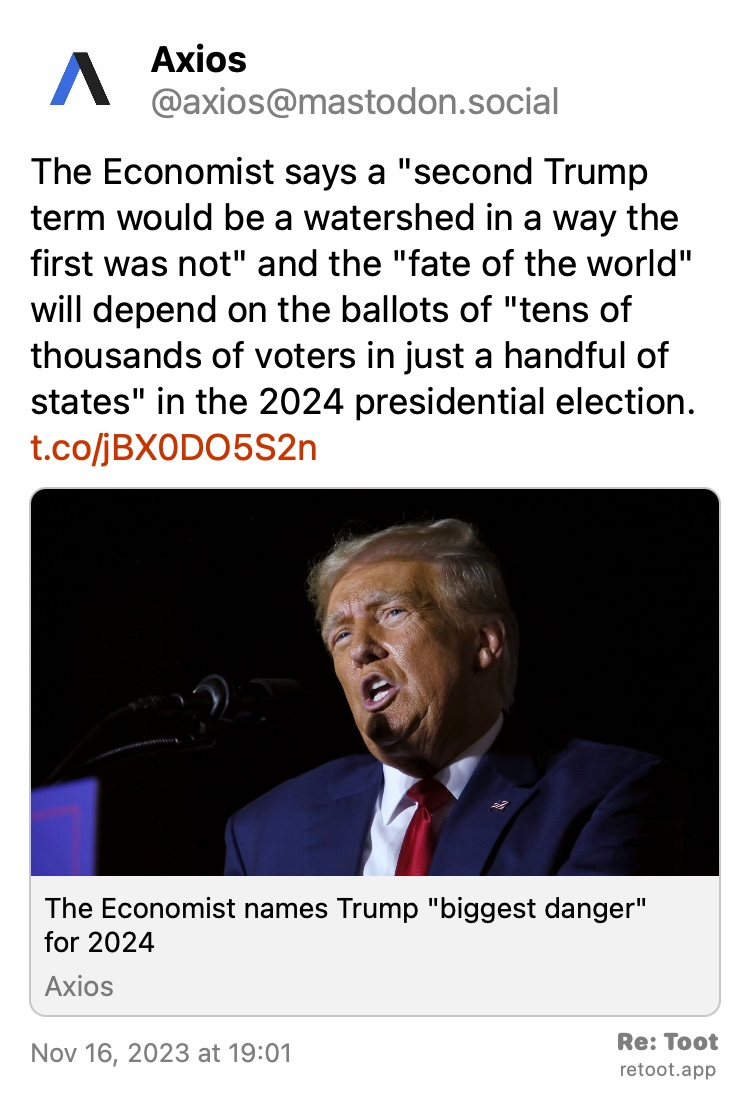
\includegraphics[keepaspectratio]{\%7B\%7Bsite.url\%7D\%7D/img/trumpthreat.jpg}}
\caption{Post by Axios. ``The Economist says a''second Trump term would
be a watershed in a way the first was not'' and the ``fate of the
world'' will depend on the ballots of ``tens of thousands of voters in
just a handful of states'' in the 2024 presidential election.
t.co/jBX0DO5S2n'' Posted on Nov 16, 2023 at 19:01}
\end{figure}

\begin{quote}
\emph{Post by Axios. ``The Economist says a''second Trump term would be
a watershed in a way the first was not'' and the ``fate of the world''
will depend on the ballots of ``tens of thousands of voters in just a
handful of states'' in the 2024 presidential election. t.co/jBX0DO5S2n''
Posted on Nov 16, 2023 at 19:01}
\end{quote}

In an
\href{https://www.axios.com/2023/11/16/economist-trump-2024-presidential?utm_source=twitter&utm_medium=social&utm_campaign=editorial}{article
posted by Axios} we have a horrible discussion of the relative danger to
the world posted by Donald John Trump. We're sleepwalking toward
disaster it seems. We'll have to wait and see what erupts, I think.

Quoting \href{https://journa.host/@w7voa/}{@w7voa@journa.host}:
\url{https://journa.host/@w7voa/111422495799436440} \#retoot

\begin{figure}
\centering
\pandocbounded{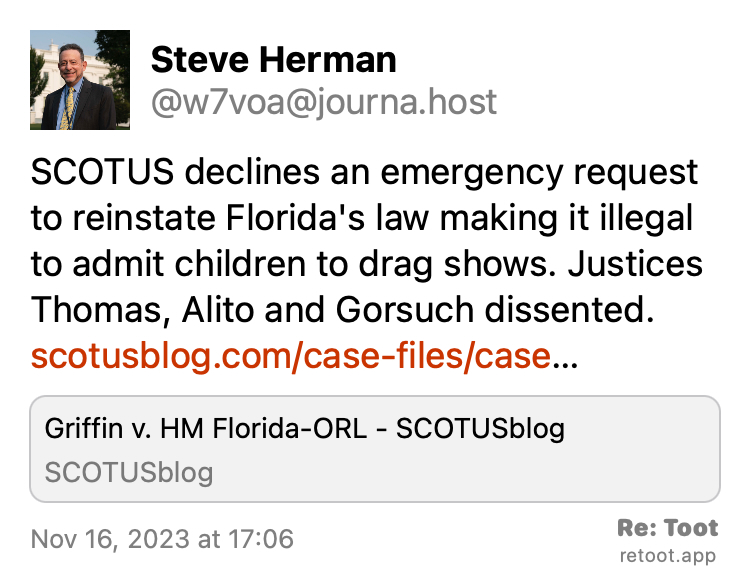
\includegraphics[keepaspectratio]{\%7B\%7Bsite.url\%7D\%7D/img/notodraglaw.jpg}}
\caption{Post by Steve Herman. ``SCOTUS declines an emergency request to
reinstate Florida's law making it illegal to admit children to drag
shows. Justices Thomas, Alito and Gorsuch dissented.
scotusblog.com/case-files/case\ldots{}'' Posted on Nov 16, 2023 at
17:06}
\end{figure}

\begin{quote}
\emph{Post by Steve Herman. ``SCOTUS declines an emergency request to
reinstate Florida's law making it illegal to admit children to drag
shows. Justices Thomas, Alito and Gorsuch dissented.
scotusblog.com/case-files/case\ldots{}'' Posted on Nov 16, 2023 at
17:06}
\end{quote}

Good! Unfortunately we've had a copycat law introduced in our state
legislature in Ohio. This might scare our goofballs in Columbus from
trying to do such a thing here.

Quoting \href{https://mastodon.social/@axios/}{@axios@mastodon.social}:
\url{https://mastodon.social/@axios/111421262780280309} \#retoot

\begin{figure}
\centering
\pandocbounded{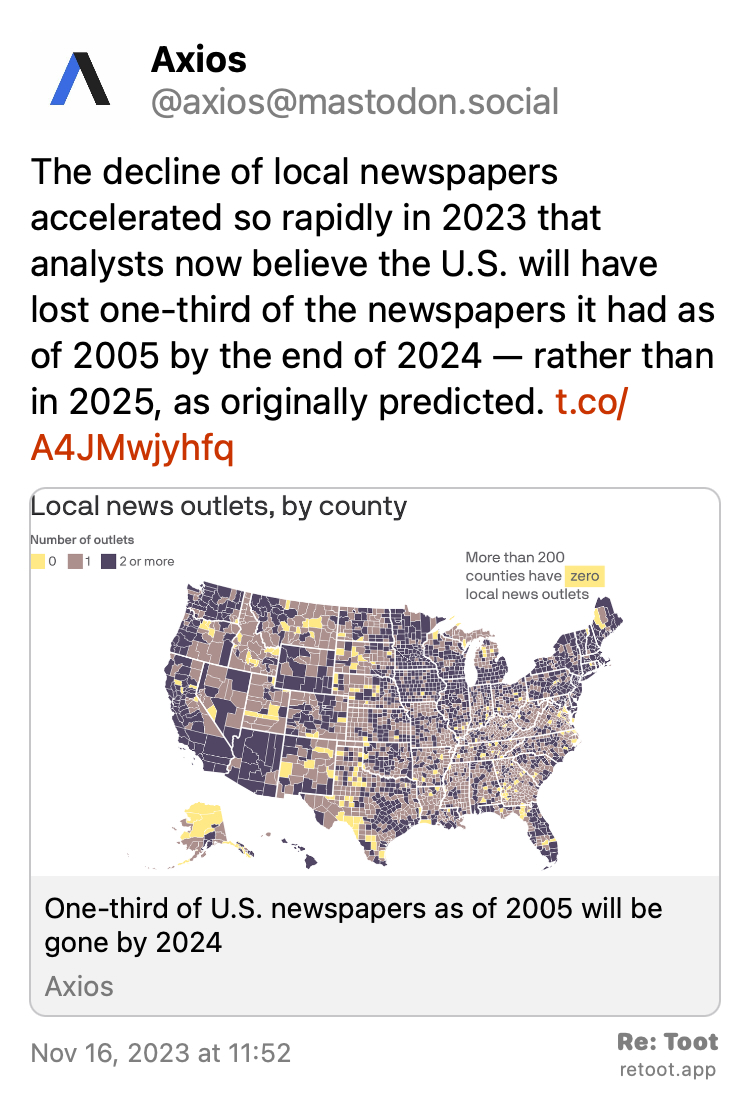
\includegraphics[keepaspectratio]{\%7B\%7Bsite.url\%7D\%7D/img/dyingnewspapers.jpg}}
\caption{Post by Axios. ``The decline of local newspapers accelerated so
rapidly in 2023 that analysts now believe the U.S. will have lost
one-third of the newspapers it had as of 2005 by the end of 2024 ---
rather than in 2025, as originally predicted. t.co/A4JMwjyhfq'' Posted
on Nov 16, 2023 at 11:52}
\end{figure}

\begin{quote}
\emph{Post by Axios. ``The decline of local newspapers accelerated so
rapidly in 2023 that analysts now believe the U.S. will have lost
one-third of the newspapers it had as of 2005 by the end of 2024 ---
rather than in 2025, as originally predicted. t.co/A4JMwjyhfq'' Posted
on Nov 16, 2023 at 11:52}
\end{quote}

In
\href{https://www.axios.com/2023/11/16/newspapers-decline-hedge-funds-research}{this
article} we see a not so happy picture painted. I do quibble with their
\href{https://localnewsinitiative.northwestern.edu/projects/state-of-local-news/explore/\#/newsNaper?state=OH&stateCode=39}{mapping}
as to Ashtabula County. Four of the five outlets they refer to are just
variant titles of the same weekly newspaper. Content differs between the
four by maybe five percent or so seemingly. In the early days of the
pandemic there was no differentiation of content whatsoever between the
four variant titles. In practical functional terms we have \textbf{one}
daily newspaper and \textbf{one} weekly newspaper. The \textbf{one}
daily newspaper is a CNHI property that is a
\href{https://www.usnewsdeserts.com/reports/expanding-news-desert/loss-of-local-news/the-rise-of-the-ghost-newspaper/}{ghost
newspaper}. As to the weekly newspaper, it covers many things but having
a weekly cover a territory equal in size to \emph{Rhode Island} means
you're missing things even if you're trying really, really hard.

Quoting \href{https://mastodon.social/@PCMag/}{@PCMag@mastodon.social}:
\url{https://mastodon.social/@PCMag/111421022142790119} \#retoot

\begin{figure}
\centering
\pandocbounded{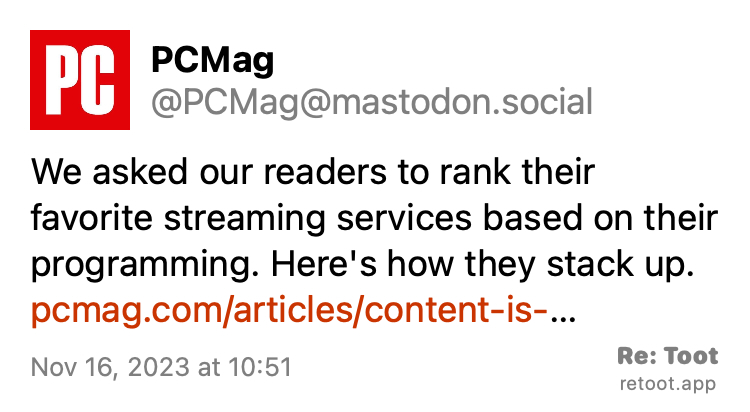
\includegraphics[keepaspectratio]{\%7B\%7Bsite.url\%7D\%7D/img/tubiwasrated.jpg}}
\caption{Post by PCMag. ``We asked our readers to rank their favorite
streaming services based on their programming. Here's how they stack up.
pcmag.com/articles/content-is-\ldots{}'' Posted on Nov 16, 2023 at
10:51}
\end{figure}

\begin{quote}
\emph{Post by PCMag. ``We asked our readers to rank their favorite
streaming services based on their programming. Here's how they stack up.
pcmag.com/articles/content-is-\ldots{}'' Posted on Nov 16, 2023 at
10:51}
\end{quote}

I just found
\href{https://www.pcmag.com/articles/content-is-king-which-streaming-services-have-the-best-selection}{this
particular article} hilarious due to how highly
\href{https://tubitv.com/}{Tubi} was ranked. Tubi is home to great films
like
\href{https://tubitv.com/movies/502449/the-creation-of-the-humanoids?start=false}{\emph{The
Humanoids}} and
\href{https://tubitv.com/movies/502446/war-between-the-planets}{\emph{War
Between The Planets}} among many other strange ones. They have a good
independent film selection, too.

Quoting \href{https://mastodon.social/@axios/}{@axios@mastodon.social}:
\url{https://mastodon.social/@axios/111424304378417459} \#retoot

\begin{figure}
\centering
\pandocbounded{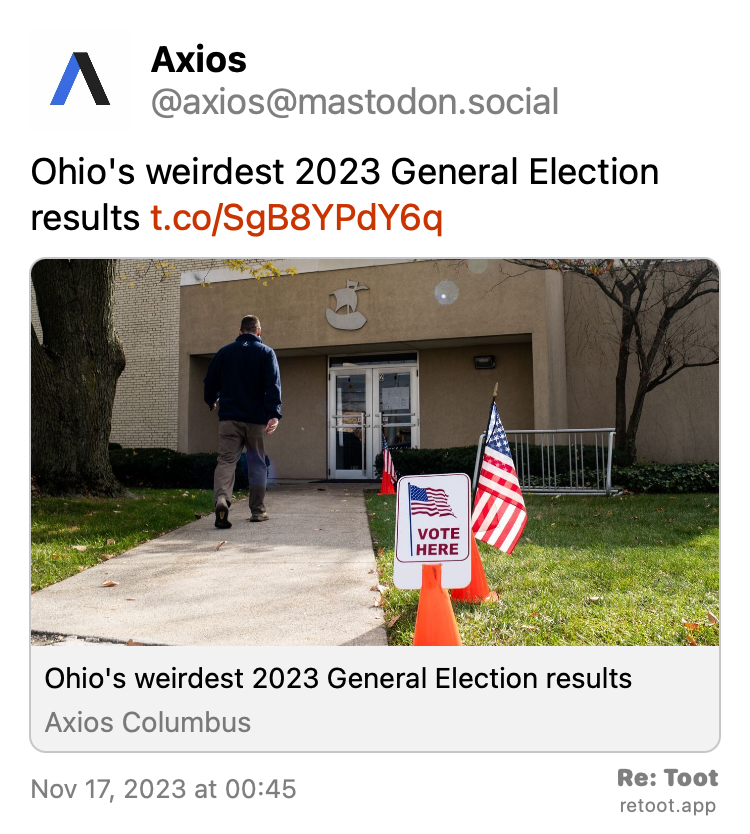
\includegraphics[keepaspectratio]{\%7B\%7Bsite.url\%7D\%7D/img/ohioweirdresults.jpg}}
\caption{Post by Axios. ``Ohio's weirdest 2023 General Election results
t.co/SgB8YPdY6q'' Posted on Nov 17, 2023 at 00:45}
\end{figure}

\begin{quote}
\emph{Post by Axios. ``Ohio's weirdest 2023 General Election results
t.co/SgB8YPdY6q'' Posted on Nov 17, 2023 at 00:45}
\end{quote}

The indefatigable Tyler Buchnan made a
\href{https://www.axios.com/local/columbus/2023/11/16/ohio-weird-election-results-2023?utm_medium=social&utm_source=twitter&utm_campaign=editorial}{quick
look at weird results} around the Buckeye State.

And, of course, the AI front continues to be odd. The prompt was:

\begin{quote}
\emph{A very friendly, very frisky, rather feminine, aerobic fitness
enthusiast from Wildemount who has a day job as a cleric for The
Traveler is having an assignation with a quite frisky female bodybuilder
who is a cleric of The Changebringer teaching at the Academy of Magic.}
\end{quote}

This was clearly a prompt rooted in the fantasy realm where I was trying
to break the parser again and get an absurd outcome. This is what was
gotten:

\begin{figure}
\centering
\pandocbounded{
\includegraphics[keepaspectratio]{\%7B\%7Bsite.url\%7D\%7D/img/ai-output-fantasy.jpg}}
\caption{Prompt used: ``A very friendly, very frisky, rather feminine,
aerobic fitness enthusiast from Wildemount who has a day job as a cleric
for The Traveler is having an assignation with a quite frisky female
bodybuilder who is a cleric of The Changebringer teaching at the Academy
of Magic.''}
\end{figure}

DALL-E 3 has problems interpreting inputs at times, though. As Harry
McCracken has been finding, these image generation AI models have
interesting problems. Quoting
\href{https://mastodon.social/@harrymccracken/}{@harrymccracken@mastodon.social}:
\url{https://mastodon.social/@harrymccracken/111427059602268734}
\#retoot

\begin{figure}
\centering
\pandocbounded{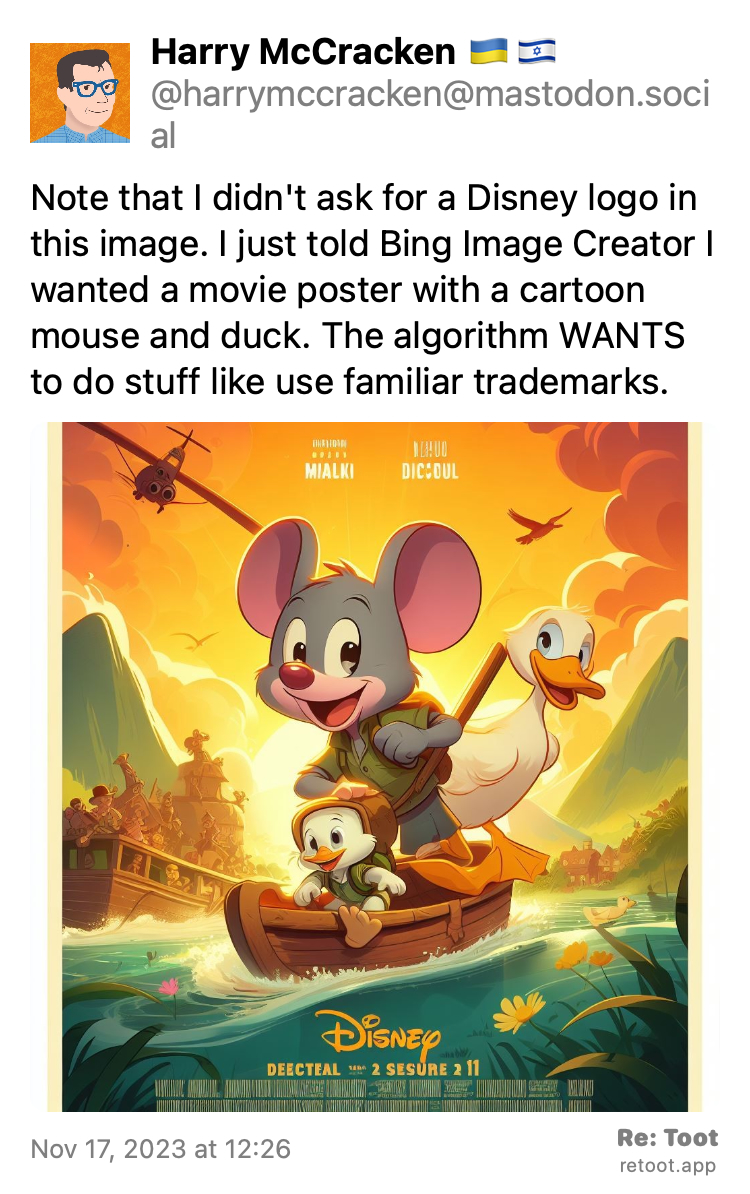
\includegraphics[keepaspectratio]{\%7B\%7Bsite.url\%7D\%7D/img/moreharrybadai.jpg}}
\caption{Post by Harry McCracken 🇺🇦🇮🇱. ``Note that I didn't ask for a
Disney logo in this image. I just told Bing Image Creator I wanted a
movie poster with a cartoon mouse and duck. The algorithm WANTS to do
stuff like use familiar trademarks.'' The post contains an image with
the following description: ``Bing Image Creator image of movie poster
with mouse, duck, and Disney logo'' Posted on Nov 17, 2023 at 12:26}
\end{figure}

\begin{quote}
\emph{Post by Harry McCracken 🇺🇦🇮🇱. ``Note that I didn't ask for a
Disney logo in this image. I just told Bing Image Creator I wanted a
movie poster with a cartoon mouse and duck. The algorithm WANTS to do
stuff like use familiar trademarks.'' The post contains an image with
the following description: ``Bing Image Creator image of movie poster
with mouse, duck, and Disney logo'' Posted on Nov 17, 2023 at 12:26}
\end{quote}

Things are getting weird as we wind down 2023\ldots{}
